%---------------------------------------------
% Ficha cutre só un folio
%--------------------------------------
\documentclass[11pt]{amsart}
\usepackage[spanish,galician]{babel}
\usepackage[utf8]{inputenc}
\usepackage{amssymb,amsmath}
\usepackage{graphicx}
%---------------------------------------------
% Ligazóns
%--------------------------------------
\usepackage{hyperref}	

%---------------------------------------------
% Marxes
%--------------------------------------
\usepackage[a4paper]{geometry}
\newgeometry{top=1cm,left=2cm,bottom=1cm}   
					%  símbolos matemáticos
%---------------------------------------------
%  interlineado	
%--------------------------------------
\renewcommand{\baselinestretch}{1.5}
%\linespread{2}


\title{Ficha  traballo }
\begin{document}
\begin{figure}[ht]
	\raggedright
	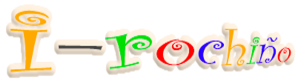
\includegraphics[width=4cm]{i-rocho.png}
\end{figure}
 \maketitle

\thispagestyle{empty} 

\begin{enumerate}
 
\item Imos  facer o circuíto máis sinxelo.  
    \begin{enumerate}
        \item  valor.
        \item Anota     
    \end{enumerate}
  
      
     \begin{table}[htp]
    \begin{center}
     \caption{Lei de Ohm en circuítos}
        \begin{tabular}{| c | c | c | c |}
            \hline
             & Voltaxe (V) &  Intensidade (A) & Resistencia ($\Omega$) \\ \hline
            Valores nominais & &\tiny{resultado da túa conta} & \\ \hline
            Valor medidos & & &   \\ \hline
        \end{tabular}
    \end{center}
    \end{table}

  
\item 
	Unha bombilla como a da nosa caixa de materiais no fondo é unha resistencia.  
    	\begin{enumerate}
        		\item  Fai mesmo exercicio anterior para a bombilla
     	 \end{enumerate}
     
 
\end{enumerate}
%
%\begin{figure}[htbp]
%\begin{center}
%
%\caption{default}
%\label{default}
%\end{center}
%\end{figure}

\end{document}  


%%%%%%%%%%%%%%%%%%%%
%  
%\item Complicámolo coas resistencias en serie.  
%\begin{enumerate}
%	\item Colocamos dúas resistencias en serie como na ficha anterior
% 	\item  Calculamos coa lei de Ohm canto debería ser a intensidade
%	\item Medimos co polímetro a intensidade que circula de verdade.
%	\item Medimos as voltaxes (caída de tensión) en cada resistencia e apuntamos noutro cadro
%    \end{enumerate}
% 
%  
% \begin{table}[htp]
%\begin{center}
% \caption{Lei de Ohm en dúas resistencias en serie}
%\begin{tabular}{| c | c | c | c | c |}
%\hline
% & Voltaxe (V) &  Intensidade (A) & Resistencia 1 ($\Omega$) & Resistencia 2 ($\Omega$)   \\ \hline
%Valores nominais & &\tiny{resultado da túa conta} & &  \\ \hline
%Valor medidos & & &  & \\ \hline
%\end{tabular}
%\end{center}
%\end{table}
%
%  
%  
% \begin{table}[htp]
% \caption{Caída de tensión en dúas resistencias en serie}
%\begin{center}
%\begin{tabular}{| c | c | c | c |}
%\hline
% (V) &  Caída de tensión na resistencia 1 & Caída de tensión na resistencia 2\\ \hline
%Voltios & &  \\ \hline
%Valor medidos & &    \\ \hline
%\end{tabular}
%\end{center}
%\end{table}


 
 
















